\documentclass[12pt]{report}
\usepackage[utf8]{vietnam}
\usepackage{titlesec}
\usepackage{titletoc}
\usepackage{listings}
\usepackage[bookmarks=true]{hyperref}
\usepackage[left=3cm,right=2cm,top=2.5cm,bottom=3cm]{geometry}
\usepackage{graphicx}
\usepackage{hyperref}
\usepackage{tikz}
\usepackage{varwidth}
\usepackage{float}
\usepackage{listings}
\usepackage{color}

\usetikzlibrary{calc}
\setlength{\parindent}{10mm}
\renewcommand{\baselinestretch}{1.3}
\graphicspath{{images/}}

\definecolor{dkgreen}{rgb}{0,0.6,0}
\definecolor{gray}{rgb}{0.5,0.5,0.5}
\definecolor{mauve}{rgb}{0.58,0,0.82}

% setup code area as listings
\lstset{frame=tb,
  language=Java,
  aboveskip=3mm,
  belowskip=3mm,
  showstringspaces=false,
  columns=flexible,
  basicstyle={\small\ttfamily},
  numbers=left,
  numberstyle=\tiny\color{gray},
  keywordstyle=\color{blue},
  commentstyle=\color{dkgreen},
  stringstyle=\color{mauve},
  breaklines=true,
  breakatwhitespace=true,
  tabsize=3
}
\renewcommand{\lstlistingname}{Mã nguồn}


% hyper setup
\hypersetup{
	bookmarks=true,
	pdftitle={Xây dựng công cụ hỗ trợ quản lý và đảm bảo chất lượng cho các phiên bản phần mềm},
	pdfauthor={Bùi Quang Cường}, % author
	pdfsubject={TeX and LaTeX},
	pdfkeywords={TeX, LaTeX, graphics, images}, % list of keywords
	colorlinks=true,       % false: boxed links; true: colored links
	linkcolor=blue,       % color of internal links
	citecolor=black,       % color of links to bibliography
	filecolor=black,        % color of file links
	urlcolor=purple,        % color of external links
	linktoc=page            % only page is linked
}

\date{}


\newpagestyle{long}
{\sethead{\thesection. \sectiontitle}{}{\subsectiontitle}\headrule
	\setfoot{}{\thepage}{}}

\begin{document}
\begin{titlepage}
	\center
	
\begin{tikzpicture}[overlay,remember picture]
		\draw [line width=3pt,rounded corners=0pt,]
		($ (current page.north west) + (25mm,-25mm) $)
		rectangle
		($ (current page.south east) + (-15mm,25mm) $);
		\draw [line width=1pt,rounded corners=0pt]
		($ (current page.north west) + (26.5mm,-26.5mm) $)
		rectangle
		($ (current page.south east) + (-16.5mm,26.5mm) $);
	\end{tikzpicture}
	
	{\large \bfseries ĐẠI HỌC QUỐC GIA HÀ NỘI\\ TRƯỜNG ĐẠI HỌC CÔNG NGHỆ}\\[1cm]
	
\includegraphics[width=0.2\linewidth]{uet}\\[1cm]
	{\Large  \bfseries Bùi Quang Cường}\\[2cm]
	{ \LARGE \bfseries XÂY DỰNG CÔNG CỤ HỖ TRỢ QUẢN LÝ VÀ ĐẢM BẢO CHẤT LƯỢNG CHO CÁC PHIÊN BẢN PHẦN MỀM}\\[0.5cm]
	\hfill\\[3cm]
	{\large \bfseries KHÓA LUẬN TỐT NGHIỆP ĐẠI HỌC HỆ CHÍNH QUY}\\	
	{\large \bfseries Ngành: Công nghệ thông tin}	
	\hfill\\[3cm]	
	{\large \bfseries HÀ NỘI - 2018}\\	
	\vfill
\end{titlepage}
	
%-----SECONDARY TITLE PAGE-----%	
\begin{titlepage}
	\center
	
\begin{tikzpicture}[overlay,remember picture]
		\draw [line width=3pt,rounded corners=0pt,]
		($ (current page.north west) + (25mm,-25mm) $)
		rectangle
		($ (current page.south east) + (-15mm,25mm) $);
		\draw [line width=1pt,rounded corners=0pt]
		($ (current page.north west) + (26.5mm,-26.5mm) $)
		rectangle
		($ (current page.south east) + (-16.5mm,26.5mm) $);
	\end{tikzpicture}
	
	{\large \bfseries ĐẠI HỌC QUỐC GIA HÀ NỘI\\ TRƯỜNG ĐẠI HỌC CÔNG NGHỆ}\\[2cm]

	{\Large  \bfseries Bùi Quang Cường}\\[2cm]		
	{ \LARGE \bfseries XÂY DỰNG CÔNG CỤ HỖ TRỢ QUẢN LÝ VÀ ĐẢM BẢO CHẤT LƯỢNG CHO CÁC PHIÊN BẢN PHẦN MỀM}\\[0.5cm]
	\hfill\\[2cm]
	{\large \bfseries KHÓA LUẬN TỐT NGHIỆP ĐẠI HỌC HỆ CHÍNH QUY}\\	
	{\large \bfseries Ngành: Công nghệ thông tin}
	\hfill\\[2cm]
	\begin{flushleft}
		{\large \bfseries Cán bộ hướng dẫn: PGS. TS. Phạm Ngọc Hùng}\\	
	\end{flushleft}
	\hfill\\[4cm]		
	{\large \bfseries HÀ NỘI - 2018}\\		
	\vfill		
\end{titlepage}

%-----THANKS-----%
\newpage
\begin{titlepage}
\begin{center}
	\textbf{\large LỜI CẢM ƠN}
\end{center}
Đầu tiên, tôi xin gửi lời cảm ơn chân thành và sâu sắc tới thầy giáo PGS. TS. Phạm Ngọc Hùng – người đã trực tiếp hướng dẫn tận tình và đóng góp những ý kiến quý báu trong suốt quá trình tôi học tập, nghiên cứu cũng như khi tôi làm khóa luận tốt nghiệp này, người đã cho tôi nhiều lời động viên, những kiến thức quý báu giúp tôi trưởng thành hơn trong cuộc sống.\\

Tôi xin gửi lời cảm ơn tới những người bạn trong tập thể K59CLC – những người đã luôn đồng hành cùng tôi suốt bốn năm qua trên mọi nẻo đường, giúp đỡ tôi mỗi khi khó khăn, chia sẻ cùng tôi mọi chuyện trong học tập và cuộc sống và góp ý cho tôi những lời khuyên chân thành giúp tôi học tập tốt hơn và hoàn thành khóa luận này.\\

Tiếp theo tôi xin gửi lời cảm ơn đến các thầy cô giảng viên Trường Đại học Công Nghệ - Đại Học Quốc Gia Hà Nội – những người đã tận tâm truyền đạt những kiến thức quý báu làm nền tảng để tôi tiếp tục đi xa hơn nữa trong lĩnh vực công nghệ thông tin.Cuối cùng, tôi xin được cảm ơn cha mẹ, anh chị và người thân, những người đã không quản khó khăn, vất vả nuôi con ăn học để con có thể phấn đấu trở thành người có ích cho xã hội.
\end{titlepage}

	
%-----ABSTRACT-----%
\newpage
\begin{titlepage}
\begin{center}
	\textbf{\large TÓM TẮT}
\end{center}
\textbf{Tóm tắt:} Mã nguồn ứng dụng trở nên lớn và phức tạp sau quá trình dài phát triển, bảo trì và nâng cấp. Vấn đề này đang dần phổ biến đối với các doanh nghiệp phát triển phần mềm, gây khó khăn trong việc kiểm soát và đảm bảo chất lượng cho các ứng dụng. Hiện nay đã có một số công cụ được đề xuất để giải quyết vấn đề trên nhưng chưa có kết quả thỏa đáng. Nghiên cứu này đề xuất các phương pháp và xây dựng một bộ công cụ toàn diện cho việc phân tích và đảm bảo chất lượng mã nguồn cho các ứng dụng doanh nghiệp sử dụng các nền tảng J2EE phổ biến Struts 2, Hibernate, Spring. Đầu tiên, mã nguồn của ứng dụng sẽ được tiền xử lý để tạo cây cấu trúc. Mỗi nút trên cây đại diện cho một thành phần mã nguồn. Tiếp theo, các nút sẽ được phân tích theo các công nghệ sử dụng trong ứng dụng để xác định mối quan hệ phụ thuộc. Cây cấu trúc này được sử dụng làm đầu vào cho việc phân tích ảnh hưởng sự thay đổi và các chức năng phân tích cấu trúc như xây dựng đồ thị dữ liệu; xây dựng kiến trúc về công nghệ, cơ sở dữ liệu; tính toán độ phức tạp mã nguồn. Phương pháp phân tích ảnh hưởng sự thay đổi được đề xuất cải tiến theo hướng tự động hóa bằng phương pháp so sánh các phiên bản mã nguồn. Hiện nay, bộ công cụ đang được triển khai thử nghiệm tại Trung tâm công nghệ và quản lý chất lượng phần mềm Viettel (VITM) và nhận được nhiều phản hồi tích cực.\\

\noindent \textit{\textbf{Từ khóa:} phân tích mã nguồn, phiên bản mã nguồn, ứng dụng doanh nghiệp}
\end{titlepage}

%-----ABSTRACT (ENGLISH)-----%
\newpage
\begin{titlepage}
\begin{center}
	\textbf{\large ABSTRACT}
\end{center}
\end{titlepage}

%-----UNDERTAKING-----%
\newpage
\begin{titlepage}
\begin{center}
	\textbf{\large LỜI CAM ĐOAN}
\end{center}
Tôi xin cam đoan rằng những nghiên cứu về phương pháp hỗ trợ quản lý và đảm bảo chất lượng cho các phiên bản phần mềm được trình bày trong khóa luận này là của tôi và chưa từng được nộp như một báo cáo khóa luận tại trường Đại học Công Nghệ - Đại học quốc gia Hà Nội hoặc bất kỳ trường đại học khác. Những gì tôi viết ra không sao chép từ các tài liệu, không sử dụng các kết quả của người khác mà không trích dẫn cụ thể.Tôi xin cam đoan công cụ hỗ trợ quản lý và đảm bảo chất lượng tôi trình bày trong khoá luận là do tôi tự phát triển, không sao chép mã nguồn của người khác. Nếu sai tôi hoàn toàn chịu trách nhiệm theo quy định của trường Đại Học Công Nghệ - Đại Học Quốc Gia Hà Nội.\\

\begin{flushright}
	\begin{varwidth}{\linewidth}\centering
		Hà Nội, ngày 26 tháng 04 năm 2018\\
		Sinh viên\\[2cm]
		Bùi Quang Cường
	\end{varwidth}
\end{flushright}
\end{titlepage}

%-----TOC-----%
\newpage
\begin{titlepage}
\tableofcontents
\end{titlepage}

%-----MAIN-----%
\newpage
\setcounter{page}{1}
\chapter{Đặt vấn đề}
Hiện nay, các ứng dụng tại các doanh nghiệp thường được phát triển trong một thời gian
dài với quy mô lớn và độ phức tạp cao. Trải qua nhiều phiên bản nâng cấp, các ứng dụng
này thường thiếu tài liệu đặc tả và thiết kế. Có thể nói tài liệu gần như duy nhất của các
ứng dụng này là mã nguồn. Trong khi đó, quá trình bảo trì và nâng cấp diễn ra thường
xuyên. Để đảm bảo chất lượng cho mỗi phiên bản mới, đội dự án cần thực hiện kiểm thử
lại toàn bộ hệ thống. Điều này là không thể bởi chi phí cho việc này rất tốn kém. Kết quả
là chúng ta không thể kiếm soát toàn bộ sự ảnh hưởng của việc thay đổi và có thể dẫn đến
nhiều rủi ro lớn cho doanh nghiệp trong quá trình vận hành. Đây là một bài toán khó tổng
quát hóa vì các giải pháp đề xuất phụ thuộc chặt chẽ vào các công nghệ được sử dụng
trong ứng dụng. Đề xuất các giải pháp và xây dựng công cụ đủ tốt để giải quyết vấn đề
nêu trên đang là một trong những thách thức lớn và nhận được sự quan tâm nghiên cứu.\\

Phân tích ảnh hưởng sự thay đổi (Change Impact Analysis - CIA) được xem là một
giải pháp để giải quyết bài toán trên. CIA có vai trò quan trọng trong các giai đoạn phát
triển, bảo trì và kiểm thử hồi quy. Đối với người quản lý và lập trình viên, CIA là công cụ
đánh giá phạm vi ảnh hưởng, ước lượng chi phí từ đó lên kế hoạch thực hiện thay đổi.
Đối với kiểm thử viên, trong quá trình kiểm thử hồi quy, CIA có thể ứng dụng vào việc
xác định những ca kiểm thử có liên quan đến phần mã nguồn chỉnh sửa, điều này giúp
giảm số lượng các ca kiểm thử cần thực hiện từ đó rút ngắn thời gian và nỗ lực kiểm thử.
Các kĩ thuật CIA được thực hiện theo hai hướng tiếp cận chính là phân tích tĩnh (static
CIA) và phân tích động (dynamic CIA) [1]. Trong thực tế, hầu hết các nghiên cứu đề xuất
các phương pháp phân tích ảnh hưởng sự thay đổi liên quan đến static CIA. Nổi bật trong
số đó là kĩ thuật CIA dựa trên sự phân loại thay đổi [2], kĩ thuật dựa vào đồ thị Call
Graph [3] và kĩ thuật dựa trên tư tưởng giao thoa sóng nước WAVE-CIA [4]. Tuy nhiên,
Các kĩ thuật CIA sử dụng đầu vào là kết quả của quá trình phân tích phụ thuộc từ ứng
dụng. Quá trình này không thể tổng quát hóa cho toàn bộ các công nghệ và nền tảng hiện
có.\\

J2EE đang là một giải pháp phổ biến được sử dụng để triển khai cho các ứng dụng
Web doanh nghiệp hiện đại. Nó bao gồm nhiều công nghệ cốt lõi như EJB, JSF, CDI,
JAX-WS, JPA, JMS, v.v và có thể tích hợp nhiều framework khác như Spring, Struts,
Hibernate, Vaddin, GWT, Play!, Grails, v.v. Để giải quyết bài toán trên cho các ứng dụng 
2
J2EE, một phương pháp kèm theo công cụ có tên JCIA [5] đã được đề xuất và xây dựng.
Tuy nhiên phương pháp này khá thô sơ và chỉ đề xuất phân tích cho một số công nghệ cốt
lõi của J2EE. Công cụ JCIA còn đơn giản, chưa được hoàn thiện và chưa mang lại tính
hiệu quả cao.\\

Dựa trên ý tưởng về phương pháp này, một phương pháp hoàn chỉnh đã được nghiên
cứu và đề xuất để thực hiện phân tích ảnh hưởng sự thay đổi cho các ứng dụng J2EE đa
nền tảng. Các framework phổ biến hiện nay: Spring, Struts, Hibernate sẽ được tập trung
hỗ trợ đầu tiên. Sau đó chúng tôi sẽ dần hoàn thiện phương pháp cho các tất cả các nền
tảng khác. Ngoài ra, chúng tôi cũng đề xuất các giải pháp khác để đem lại nhiều góc nhìn
khách quan về hệ thông ứng dụng như xây dựng dòng dữ liệu, tái hiện thiết kế kiến trúc
hệ thống và cơ sở dữ liệu, và tính toán độ phức tạp mã nguồn. Một bộ công cụ được phát
triển như là phiên bản tiếp theo của công cụ JCIA để thực hiện các giải pháp đã đề xuất.\\

Phần còn lại của báo cáo được cấu trúc như sau. Phần 2 trình bày các phương pháp
thực hiện về tiền xử lý mã nguồn; phân tích phụ thuộc cho các công nghệ Struts 2, Spring,
Hibernate; quản lý các phiên bản phân tích; xây dựng dòng dữ liệu và cuối cùng là biểu
diễn các góc nhìn kiến trúc của ứng dụng. Tiếp theo, phần 3 trình bày bộ công cụ đảm
bảo chất lượng JCIA-VT, và kết quả đạt được qua thực nghiệm phân tích. Cuối cùng,
phần 4 tóm tắt các kết quả đạt được, kết luận, hạn chế và hướng nghiên cứu phát triển
trong tương lai.


\newpage	
\chapter{Lý thuyết phân tích ảnh hưởng sự thay đổi}
Bảo trì phần mềm luôn được coi là hoạt động khó và tiêu tốn chi phí nhiều nhất trong quá trình phát triển phần mềm. Các sản phẩm phẩm phần mềm liên tục thay đổi và thích nghi với các yêu cầu thay đổi để phù hợp với nhu cầu của người dùng. Khi các thay đổi được thực hiện, nó sẽ gây ra các ảnh hướng không lường trước được, và có thể gây ra các tác động làm mất sự nhất quán đối với các thành phần của phần mềm.\\

Phân tích ảnh hưởng sự thay đổi (Change Impact Analysis - CIA) bao gồm một bộ các kỹ thuật giúp xác định sự ảnh hưởng của các thay đổi được đề xuất tới các thành phần phần mềm. Nó đóng vai trò quan trọng trong quá trình phát triển, bảo trì phần mềm và kiểm thử hồi quy.\\

CIA có thể được sử dụng trước hoặc sau khi thực hiện thay đổi. Trước khi thực hiện thay đổi, CIA có thể được sử dụng để tiên đoán ảnh hưởng sự thay đổi và ước tính chi phí. Sau khi thay đổi được thực hiện, CIA có thể được ứng dụng để lựa chọn các ca kiểm thử cho quá trình kiểm thử hồi quy.\\

\section{Các phương pháp phân tích ảnh hưởng sự thay đổi}
\begin{figure}[h]
	\centering
	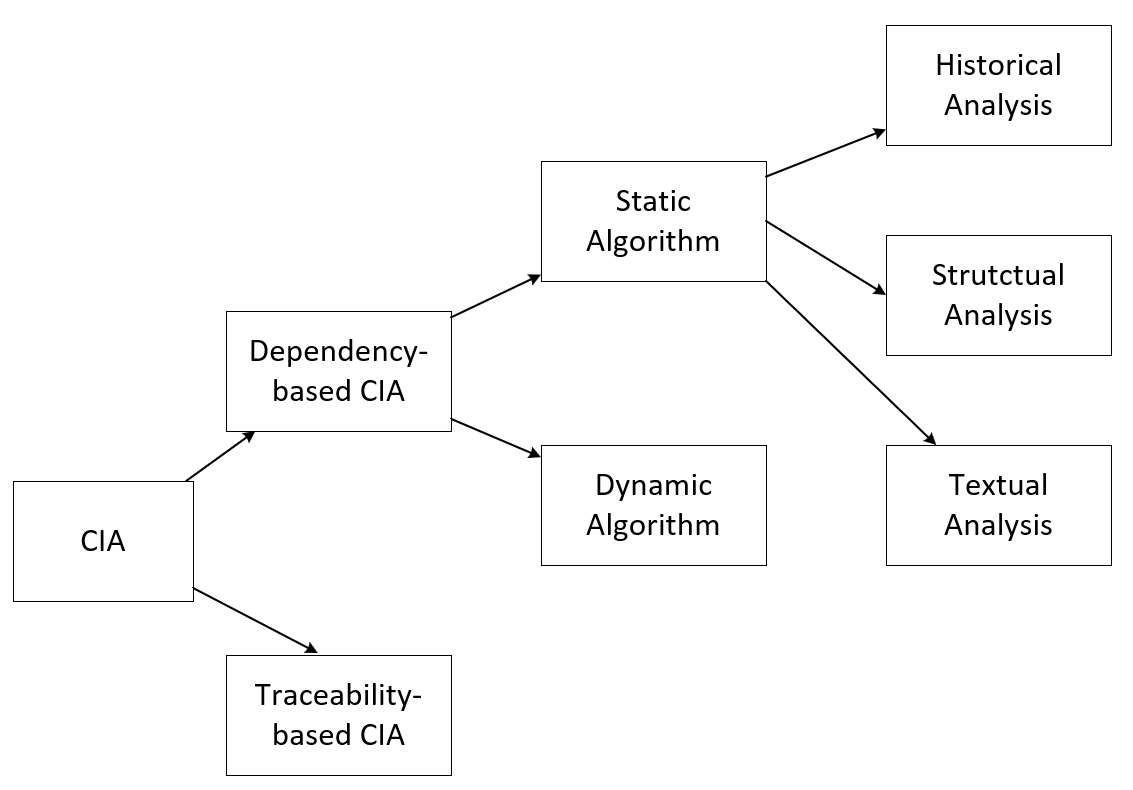
\includegraphics[scale=0.5]{CIA-hierarchy}
	\label{fig:cia-hierarchy}
	\caption{Các phương pháp CIA}
\end{figure}

Trong hơn 30 năm qua, đã có nhiều kỹ thuật CIA được nghiên cứu và đề xuất. Hình \ref{fig:cia-hierarchy} mô tả về các phương pháp CIA hiện nay đã được đề xuất. Một số phương pháp CIA dựa trên phân tích sự truy vết (traceability-based CIA) trong khi một số khác tập trung phân tích các mối quan hệ phụ thuộc (dependency-based CIA) để xác định các ảnh hưởng. Traceability-based CIA sẽ cố gắng truy vết mối liên kết giữa các phần tử trong từng mức trừu tượng với các thành phần tương ứng ở các mức khác (các mức trừu tượng: yêu cầu, tài liệu đặc tả, thiết kế, mã nguồn, ca kiểm thử). Mục tiêu của nó là gắn kết các thể hiện ở mỗi mức trừu tượng khác nhau của các đối tượng phần mềm (ví dụ: tài liệu thiết kế với mã nguồn). Trong khi đó, Depedency-based CIA tập trung xác định các mối quan hệ phụ thuộc của các thành phần trong cùng một mức trừu tượng (ví dụ: mối quan hệ giữa các lớp, phương thức, thuộc tính trong mã nguồn). Depedency-based CIA thường được áp dụng ở mức trừu tượng chi tiết hơn Traceability-based CIA.\\

Để thực hiện Depedency-based CIA, ta có thể sử dụng hai phương pháp là phân tích tĩnh và động. Phân tích động sẽ yêu cầu thực thi ứng dụng, nó sẽ thu thập các thông tin trước, trong và sau khi chạy để xác định các mối quan hệ phụ thuộc. Phương pháp này mang lại chính xác cao nhưng đòi hỏi sự phức tạp và tốn kém. Bên cạnh đó, các phương pháp phân tích tĩnh dễ thực hiện và ít tốn kém. Chúng tập được thực hiện ngay trên mã nguồn phần mềm. Có thể chia các phương pháp tĩnh này thành ba loại chính: Phân tích dựa trên lịch sử được thực hiện bằng cách khai phá thông tin từ nhiều phiên bản tiến hóa của phần mềm, phương pháp thường cho nhiều kết quả dự đoán nhầm, nhiều phần tử ảnh hưởng dự đoán thật sự không bị ảnh hưởng; Phân tích ngữ nghĩa dựa trên việc trích xuất thông tin từ việc phân tích nội dung comment hoặc các định danh (ví dụ: tên biến, phương thức); Nổi trội nhất trong đó là phân tích cấu trúc, phương pháp này tập trung phân tích tĩnh cấu trúc của chương trình, xác định các mối quan hệ giữa các thành phần và xây dựng đồ thị phụ thuộc.\\

\section{Quy trình phân tích ảnh hưởng sự thay đổi}
\begin{figure}[h]
	\centering
	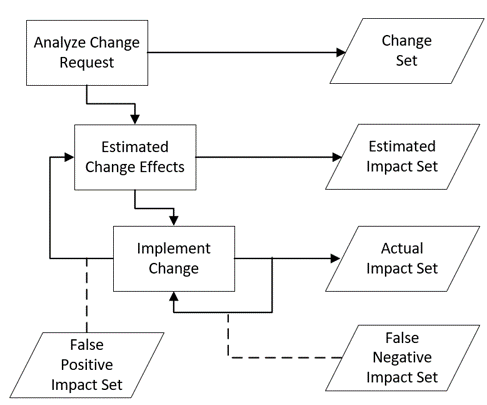
\includegraphics[scale=0.8]{CIA-process}
	\label{fig:cia-process}
	\caption{Quy trình chung CIA}
\end{figure}

Các loại thay đổi trong mã nguồn có thể chia làm hai loại chính là thay đổi cấu trúc và thay đổi lô-gíc. Thay đổi cấu trúc là các thay đổi liên quan đến các thành phần trong mã nguồn. Cụ thể đối với ngôn ngữ Java, thay đổi cấu trúc có thể là thay đổi về phạm vi truy cập, kiểu, tên của một thuộc tính hoặc thay đổi chữ kí của một phương thức. Thay đổi lô-gíc là thay đổi về thuật toán, các câu lệnh. Chúng thường là những thay đổi nằm trong thân phương thức.\\

Một thay đổi được thực hiện có thể gây ảnh hưởng không mong muốn đến những thành phần mã nguồn khác. Mục tiêu của các kỹ thuật CIA là xác định những thành phần ảnh hưởng. Hình \ref{fig:cia-process} thể hiện toàn bộ quy trình CIA. Phân tích ảnh hưởng sự thay đổi được bắt đầu bằng việc phân tích yêu cầu thay đổi để xác định được tập các thành phần thay đổi (Change Set - CS). Thông qua thuật toán CIA, các thành phần ảnh hưởng sẽ được phán đoán (Estimated Impact Set - EIS). EIS chính là đầu ra cuối cùng của quá trình CIA.\\

Phương pháp CIA hiệu quả là phương pháp giúp tìm ra được tập ảnh hưởng dự đoán gần nhất với tập ảnh hưởng thực tế khi thực hiện thay đổi (Actual Impact Set - AIS). Khi so sánh giữa EIS và AIS ta, có tập các thành phần ảnh hưởng tiên đoán nhầm (False Negative Impact Set - FNIS) và tập các thành phần ảnh hưởng tiên đoán thiếu (False Positive Impact Set - FPIS). Để đánh giá sự hiệu quả của một phương pháp CIA, người ta dùng hai độ đo là độ chính xác (Precision - P) và Recall - R, được tính theo các công thức \ref{exp:cia-precision} và \ref{exp:cia-recall}. Độ chính xác càng cao, tập FNIS sẽ càng bé, ta ít phải chú ý đến những thành phần không cần thiết. Độ hồi tưởng cào cao, tập FPIS càng bé, giúp ta phát hiện nhiều thành phần bị ảnh hưởng hơn giúp giảm số lỗi tiềm ẩn sau khi áp dụng phương pháp CIA.\\

\begin{equation}
	Precision = \frac{|EIS \cap AIS|}{EIS}
	\label{exp:cia-precision}
\end{equation}
\\
\begin{equation}
	Recall = \frac{|EIS \cap AIS|}{AIS}
	\label{exp:cia-recall}
\end{equation}


\newpage
\chapter{Phương pháp phân tích phụ thuộc cho các ứng dụng J2EE}
\section{Tiền xử lý mã nguồn ứng dụng J2EE}
\textbf{Định nghĩa:} (\textit{Cây cấu trúc}) Cho mã nguồng ứng dụng J2EE, một cây cấu trúc của mã nguồn này được định nghĩa $T = (V, E)$ với $V = \{v_1, v_2,..., v_k\}$ là tập nút đại diện cho các thành phần trong mã nguồn như thư mục; tệp; lớp, phương thức, thuộc tính (Java); thẻ (XML-based); v,v. $E = \{(v_i, v_j) | v_i,v_j \in V\}$ là tập các cạnh. Mỗi cạnh $(v_i,v_j)$ đại diện cho quan hệ phụ thuộc giữa $n_i$ và $n_j$ có nghĩa là $n_i$ phụ thuộc vào $n_j$.\\

Các ứng dụng doanh nghiệp J2EE, ngoài sử dụng mã nguồn Java còn nhiều định dạng mã nguồn khác để đảm nhiệm vai trò cho tầng \textit{View} và các thành phần cấu hình ứng dụng như XML, JSP, XHTML, FreeMarker,...Với mỗi một định dạng lại có cấu trúc và cú pháp khác nhau, tuy nhiên ta có thể phân loại thành hai nhóm là mã nguồn Java và mã nguồn XML-based (mã nguồn có cú pháp dựa trên định dạng XML). Bộ tiền xử lý cần biến đổi những mã nguồn này về định dạng chung là cây cấu trúc, các nút trên cây cấu trúc cần chứa những thông tin cần thiết cho việc phân tích phụ thuộc cũng như cây cần được thiết kế để tối ưu cho việc duyệt và tìm kiếm các nút trên cây dễ dàng.\\

\subsection{Tiền xử lý cho mã nguồn Java và mã nguồn định dạng XML}
Hình \ref{fig:preprocess} thể hiện phương pháp để tiền xử lý mã nguồn ứng dựng J2EE. Hai phương pháp chính được đề xuất để thực hiện tiền xử lý cho mã nguồn Java và mã nguồn XML-based. Một phương pháp duyệt thư mục cũng cần được đề xuất và thực hiện nhằm tìm ra các tệp chứa mã nguồn Java và XML-based trong mã nguồn ứng dụng.\\

\begin{figure}[h]
	\centering
	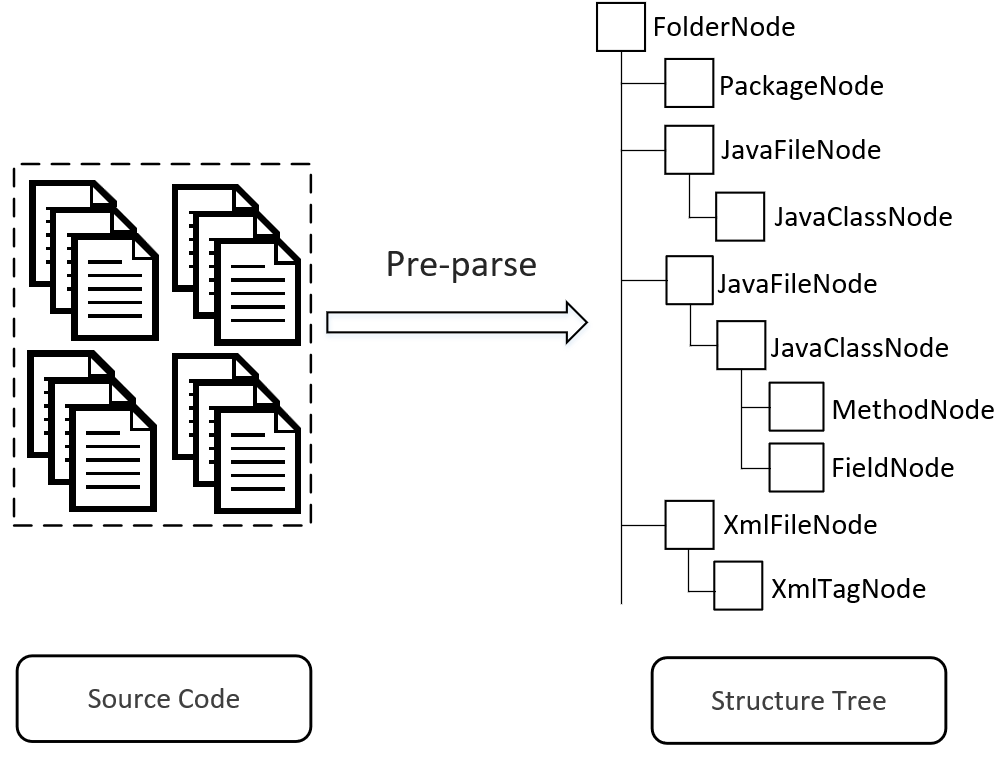
\includegraphics[scale=0.7]{preprocess}
	\label{fig:preprocess}
	\caption{Phương pháp tiền xử lý mã nguồn}
\end{figure}

Đầu tiên, ta thực hiện duyệt toàn bộ cấu trúc các thư mục và tệp trong mã nguồn ứng dụng. Ta có thể sinh được cây cấu trúc cơ bản gồm các nút thư mục và nút tệp. Tiếp theo, ta duyệt tìm tất cả các nút tệp trên cây. Các tệp mã nguồn có phần mở rộng \textit{.java} sẽ được phân tích  để thu thập thông tin và tạo các nút con tương ứng với các thành phần mã nguồn Java đó (lớp, thuộc tính, phương thức). Các thông tin của các thành phần này cũng cần được thu thập (ví dụ: đối với phương thức cần thu thập thông tin về kiểu trả về, mức truy cập, tên phương thức, danh sách các tham số). Hiện nay có một thư viện mã nguồn mở Java có tên Java Development Tools \footnote{https://www.eclipse.org/jdt/} đã hỗ trợ việc phân tích và thu thập thông tin cho các tệp mã nguồn Java. Tuy nhiên đầu ra của thư viện này chứa khá nhiều thông tin không cần thiết. Ta chỉ cần trích xuất những thông tin cần thiết để thêm vào cây cấu trúc. Các tệp mã nguồn có phần mở rộng \textit{.xml, .jsp, .html} sẽ xử lý bởi cùng một phương pháp tiền xử lý cho định dạng mã nguồn dựa trên XML. Kết quả đầu ra sẽ là các nút tương ứng với các thẻ XML có trong tệp. Các nút này cũng cần chứa toàn bộ thông tin của thẻ đấy, bao gồm các thuộc tính và nội dung của thẻ.\\

\subsection{Định danh cho các nút trên cây cấu trúc}
Cây cấu trúc là dữ liệu được sử dụng xuyên suốt trong các quá trình phân tích. Sẽ có rất nhiều hoạt động phân tích cần đến việc tìm kiếm và truy xuất dữ liệu của các nút trên cây. Vì thế việc định danh cho các nút trên cây là một việc rất quan trọng. Phương pháp đề xuất là định danh bằng đường dẫn tuyệt đối của nút. Đường dẫn tuyệt đối của mỗi nút trên cây sẽ được tạo thành bởi tên lần lượt của các nút cha và tên của nó, ngăn cách bởi kí tự gạch chéo (\texttt{/}). Với hầu hết các nút đại diện trong thành phần mã nguồn sẽ có đường dẫn tuyệt đối duy nhất, ta có thể thực hiện \textit{Indexing} các nút trên cây phục vụ cho việc tìm kiếm nhanh. Tuy nhiên, trong một số trường hợp, dùng tên các nút để tạo thành đường dẫn tuyệt đối sẽ có thể cho cùng một kết quả đối với nhiều hơn một nút.\\

\begin{lstlisting}[language=Java,
caption={Ví dụ chồng hàm trong Java},label={code:java-overloading}]
package vn.sample.manager.BookManager;
import vn.sample.model.Boook;
import vn.sample.model.Author;
public class BookManager {
	//...	
	public void addBook(Book newBook) {
		//...
	}
	public void addBook(String bookName, Author author) {
		//...
	}
}
\end{lstlisting}

Ví dụ như ở Mã nguồn \ref{code:java-overloading} thể hiện sự chồng hàm của phương thức \texttt{addBook()}. Nếu chỉ sử dụng tên của phương thức thì ta sẽ không định danh cho các các nút tương ứng với hai phương thức này được. Do vậy ta cần sử dụng cả thông tin về các tham số của chúng để tạo đường dẫn tuyệt đối. Bao gồm cả tên, kiểu và thứ tự của các tham số này trong phần khai báo phương thức. Kết quả ta được hai đường dẫn tuyệt đối có thể đại diện cho sự riêng biệt của các nút phương thức Java này.\\

\begin{verbatim}
vn/sample/manager/BookManager.java/BookManager/addBook(vn.sample.model.Book_newBook)
vn/sample/manager/BookManager.java/BookManager/
addBook(java.lang.String_bookName,java.lang.String_author)
\end{verbatim}

Hoặc đối với mã nguồn dựa trên định dạng XML như ở Mã nguồn \ref{code:html-example}, nếu dùng tên thẻ để làm đường dẫn tuyệt đối thì hai phần tử \texttt{h1} sẽ có chung giá trị là \texttt{web/hello.html/html/body/h1}. Để định danh cho hai phần này, ta sẽ dùng thêm các thuộc tích đặc biệt là tọa độ thẻ mở của chúng trong mã nguồn. Ví dụ với phần \texttt{h1} đầu tiên, sẽ có tọa độ số dòng là 3, số cột là 12 cho nên đường dẫn tuyệt đối của nó sẽ là \texttt{web/hello.html/html/body/h1:3:12}. Đường dẫn mới này sẽ giúp phân biệt phần tử này với phần liền kề với đường dẫn \texttt{web/hello.html/html/body/h1:4:12}. Thật may mắn nền tảng Java cung cấp sẵn một thư viện giúp chúng ta phân tích các tệp có định dạng XML và lấy được tọa độ của các phần tử này. Nó là SAXParser, nó sẽ giúp tiết kiệm công sức rất nhiều trong việc tiền xử lý phần mã nguồn này.\\

\begin{lstlisting}[language=XML,
caption={Ví dụ mã nguồn HTML},label={code:html-example}]
<html>
	<body>
		<h1>Hello!</h1>
		<h1>I am writing this line with Latex.</h1>
	</body>
</html>
\end{lstlisting}

\subsection{Làm mịn cây cấu trúc}



\section{Phân tích phụ thuộc Java Core}
\section{Phân tích phụ thuộc Struts}

\chapter{Phương pháp quản lý các phiên bản}
\section{So sánh hai phiên bản}
\chapter{Phương pháp phân tích ảnh hưởng sự thay đổi}
\chapter{Thực nghiệm và triển khai}
\chapter{Kết luận}
\end{document}
